\chapter{实验与评估}

基于上述实现,本设计完成了对rel4系统中,基于taic的异步系统调用优化。为验证系统的功能正确性与性能优化情况,本设计编写了测试用例并FPGA上进行实验验证。本章将对实验的情况进行讲解,并对实验结果进行分析。

\section{测试环境与平台}

本实验采用的宿主机环境如下表所示:

\begin{table}[htbp]
\centering
\renewcommand{\arraystretch}{1.2}
\begin{tabular}{|l|l|}
\hline
\textbf{CPU} & AMD Ryzen 7 5800H with Radeon Graphics 3.20 GHz \\
\hline
\textbf{操作系统} & Windows 11 专业版,操作系统版本	26100.3915 \\
\hline
\textbf{系统架构} & x86\_64 \\
\hline
\textbf{内存大小} & 32 GB \\
\hline
\end{tabular}
\caption{宿主机环境配置}
\label{tab:experiment-platform}
\end{table}


本实验采用的虚拟机环境如下表所示:

\begin{table}[htbp]
\centering
\renewcommand{\arraystretch}{1.2}
\begin{tabular}{|l|l|}
\hline
虚拟机软件 & VMware® Workstation 17 Pro \\
\hline
虚拟机版本 & 17.5.0 build-22583795 \\
\hline
虚拟机操作系统 & Ubuntu 24.04.1 LTS \\
\hline
虚拟机内核版本 & Linux 6.11.0-25-generic \\
\hline
虚拟机核心数与内存大小 & 4核心,8GB \\
\hline
\end{tabular}
\caption{虚拟机环境配置}
\label{tab:vmware-platform}
\end{table}

本实验在FPGA上对异步系统调用性能进行评估验证,开发板部分信息如下:

% 表:开发板及FPGA型号信息
\begin{table}[htbp]
\centering
\renewcommand{\arraystretch}{1.2}
\begin{tabular}{|l|l|}
\hline
\textbf{开发板型号} & AXU15EG \\
\hline
\textbf{FPGA型号} & Zynq UltraScale+ XCZU15EG-2FFVB1156 MPSoC \\
\hline
\multicolumn{2}{|c|}{FPGA开发板RISC-V子系统参数表} \\
\hline
核心数 & 2 \\
\hline
频率 & 100 MHz \\
\hline
BTB入口数量 & 40 \\
\hline
L2缓存大小 & 2 MB \\
\hline
内存大小 & 2 GB \\
\hline
\end{tabular}
\caption{FPGA 开发板基本信息}
\label{tab:fpga-info}
\end{table}

\section{功能测试}

\subsection{taic调用测试}

本测试用于测试将taic适配进系统并允许用户线程访问后,是否能正常使用全局队列的各项功能。测试模拟用户线程进行任务的入队出队操作。测试中,线程使用硬件调度器分配一个全局队列,然后将100个任务入队,再将100个任务出队。

测试结果如下图所示

% 插图

由结果可知,测试成功将100个队列入队并出队,测试结果与预期相符,说明用户线程使用硬件能力正常。

\subsection{缓冲区读写测试}

本测试用于测试共享缓冲区的读写功能是否正常。测试模拟用户协程申请缓冲区索引并写入数据,内核服务协程从缓冲区读取数据并进行回复。测试时,用户协程向缓冲区写入字符串"message from usermode",内核协程拿到数据后回复"message from kernel"。

测试结果如下图所示

% 插图

有结果可知,用户协程与内核协程成功利用缓冲区进行通信,索引分配回收正常。

\subsection{异步系统调用测试}

本测试分别测试进行硬件优化后,Rel4系统中原有的各种异步系统调用功能是否正常。分别为输出类系统调用、通知类系统调用和内存映射类系统调用。



\subsection{输出类async\_sycall功能性测试}

输出类系统调用测试用例如下:

\begin{enumerate}
  \item 调用 \texttt{PutChar} 异步系统调用输出一个字符 `'X'`。
        预期结果: 控制台输出字符 `'X'`,并在日志中记录系统调用被调度。

  \item 调用 \texttt{PutString} 异步系统调用输出字符串 `"11111"`。
        预期结果: 控制台输出字符串 `"11111"`,日志显示异步系统调用调度信息。
  \item 调用 \texttt{RISC-VGetPageAddress} 异步系统调用获取目标虚拟地址 \texttt{vaddr} 所在页帧的物理地址,并通过日志输出。\\
        预期结果:日志记录异步系统调用触发,并显示页帧的物理地址,物理地址应与同步调用结果一致
\end{enumerate}

测试结果如下图所示:

\subsubsection{通知类系统调用}



\subsubsection{内存映射类系统调用}





\section{性能测试}

\subsection{测试对象选取}

本实验中选取内存映射(RISC-VPageMap)与取消映射(RISC-VPageUnmap)两个系统调用作为测试对象并设计实验场景。在基于 RISC-V架构的rel4微内核操作系统中,内存空间的管理权下放至用户态程序,用户负责页表的维护与内存区域的动态分配与释放。因此,用户态程序在运行过程中必须频繁地调用 RISC-VPageMap 和 RISC-VPageUnmap,以实现对虚拟地址空间的有效控制。因此,将二者作为本实验的测试对象,可以用于评估异步系统调用的性能。

\subsection{性能测试流程}

本实验中,测试会模拟线程多次映射物理页帧与解除物理页帧的情况。映射与解除映射时分别调用异步系统调用RISC-VPageMap与RISC-VPageUnmap。测试程序首先会初始化一个线程并为其赋予内存分配能力。随后,线程生成一定数量的物理页框供测试时映射。

为表征系统在不同并发度下的性能表现,实验设置了1、2、4、8、16、32、64、128及256多组并发度。对于每个并发度,测试程序会生成对应数量的协程。每个协程对同一页框执行10轮调用操作,每轮包括一次页帧映射与解除映射。

测试分别基于现有实现和Rel4原有的实现进行,以此对比引入taic硬件调度器前后的性能差异。此外,为进行完整的性能评估,实验使用同步系统调用作为对照。同步测试中,使用单线程循环进行系统调用,对页框进行映射与解除映射。系统调用总次数与异步调用相同。

性能评估采用以下两个指标:

1. 平均耗时

在异步测试中,该指标为从所有协程启动运行时,到所有协程均完成系统调用后所有的总时间与系统调用次数的比值。其反应异步过程中,等效的单次用时。

在同步测试中,该指标为第一次系统调用开始,到最后一次系统调用结束所有的总时间与系统调用次数的比值。

2. 陷入频率

在测试Rel4原有实现的性能时,该指标为平均每次异步系统调用中,需要陷入内核唤醒内核中协程的次数。

在测试引入硬件调度能力后,该指标为使用硬件唤醒内核中协程的次数。

测试整体的流程如下图:



\subsection{实验结果与评估}

该性能测试结果如下

\begin{figure}[htbp]
  \centering
  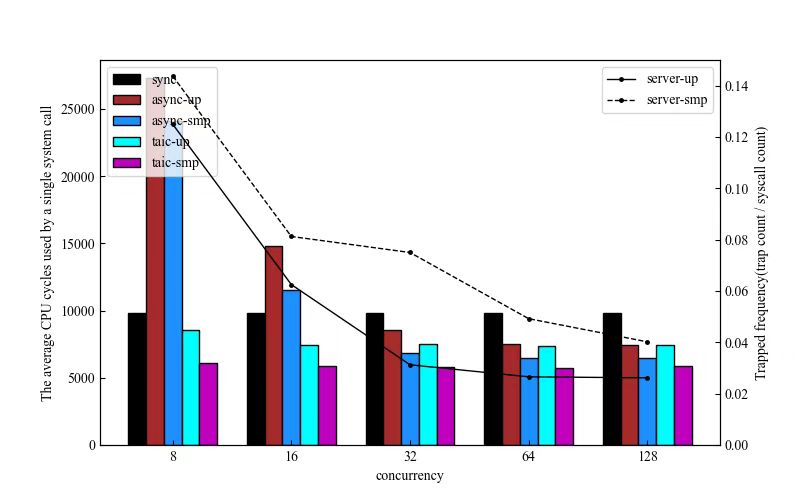
\includegraphics[width=0.8\textwidth]{images/async_syscall.jpg}
  \caption{异步系统调用性能测试结果}\label{asyncSyscall}
\end{figure}

\subsubsection{平均用时分析}

从结果中可以看出,在所有并发度下,使用taic优化后的异步系统调用平均用时均小于优化前原Rel4系统中的实现。这是由于taic降低了异步运行时引入所造成的开销。根据3.x章节中的分析,taic的使用取代了用户态中断与内核态陷入,减少了大部分原有实现中造成性能瓶颈的上下文切换。测试结果体现了优化后异步系统调用的性高效性与可用性。

由柱状图中可以看出,在并发度为8以下时,原异步实现平均用时显著高于同步,尤其在并发度为1时,平均用时大约为75000个时钟周期,约为同步调用的3倍。而优化后的异步系统调用耗时仅15000个时钟周期,有大幅度的降低。这是由于在低并发下,原有实现中内核中的异步系统调用处理协程与用户线程中的分发协程因为没有足够数量的处理请求,大多处于空闲阻塞状态,这导致平均每次调用所需的唤醒频次较高。而taic硬件的使用针对这一问题进行了优化,因此在低并发下的性能有较大的提高。

随之并发度的不断增加,所有方案的平均用时均有下降趋势,但使用taic优化后,平均用时仍具有最低的平均用时。这是由于并发数量的增加均分了内核处理时用户协程的等待时间。但并发度32以上,使用taic优化后的平均用时变化较小。这是由于并发的提高通过减少唤醒频次,减小了上下文切换的开销。引入taic后,取消了上下文切换的过程,因此优化后的平均用时随并发的增加变化较小。

在并发度为8以前,优化后异步系统调用的性能仍高于同步,这是由于异步功能的引入仍具有一定的开销,低并发下缺少足够数量的并发请求来均摊异步功能所造成的额外开销。

\subsubsection{陷入频率分析}

图中折线图部分展示了系统调用的陷入频率。

经过对实验结果的分析可知,不论在单核还是多核的测试环境下,采用优化后的异步系统调用模型的陷入频率均呈现出随着并发度提升而持续下降的趋势。如图中所示,在单核环境下,异步系统调用的陷入频率从初始并发度8时的约0.06开始,逐步下降至并发度128时的约0.02,下降幅度超过66\%;而在多核环境下,该频率最初达到约0.14,在并发度达到64后开始趋于稳定,最终在并发度128时下降至约0.04,整体下降幅度达到70\%以上。

造成这一现象的主要原因是,随着并发度的增加,用户态线程发起系统调用的整体速率提高,导致内核中协程的处理量增加。内核中的处理协程进入较长时间的持续运行状态,使得大多数系统调用请求可以被协程直接响应,无需阻塞或等待唤醒,从而显著减少了主动唤醒的次数。

\section{两种中断注册机制的对比}

为验证taic两种注册机制对异步性能的影响,本实验为两种实现方式进行了对比实验,分别测试在一次性注册与持续性注册下异步系统调用的平均用时。

% 插图

实验结果显示,两种中断注册机制在系统调用性能方面存在显著差异,其中持续性注册机制在所有并发条件下均表现出更优的性能。特别是在高并发环境下,持续性注册机制的优势更加明显,其平均系统调用用时显著低于单次注册机制。

随着并发度的提升,单次注册机制的平均调用用时呈现持续上升趋势,而持续性注册机制则保持相对稳定,特别是在并发度为64以上时,单次注册机制的平均系统调用延迟迅速上升,远高于持续性注册方式。

造成此现象的原因是,两种机制对taic中接受方注册的方式不同。单次注册机制在每次阻塞前均注册一次信号接收。这种实现虽然较为通用,但为了避免内核与用户态线程同时读写硬件寄存器而造成冲突,硬件接口层需对相关函数添加互斥锁进行保护。该互斥锁在低并发下影响较低,但在高并发场景中有较显著的性能影响。随着并发线程数的增加,频繁的争用互斥锁会导致CPU大部分时间在无意义的等待中。

而持续性注册机制在异步系统调用注册时就完成了接收方的注册,并保持注册状态。该方法下整个线程运行期间,内核无需再次进行注册操作,省去了互斥锁操作的时间成本。该机制避免了高并发情况下的冲突问题,使得优化后的异步运行时在高并发下仍有较低开销。

综上所述,在本设计中,持续性中断注册机制具有更好的性能表现,尤其在高并发场景下优势更为明显。因此,本设计最终采用持续性注册机制作为默认实现,以充分发挥硬件调度器在异步系统调用中的优势。

\section{本章小结}
